% Design study report -- Photonic Integrated Circuits, Aarhus University
% Build:  latexmk -pdf report.tex      (pdflatex + bibtex)
% Figures and Table 1 are generated from the simulation results by
%   Photonics/adc-emode-study/report_figures.py
% Rerun that script after a new simulation run, then rebuild this file.

\documentclass[11pt,a4paper]{article}

\usepackage[utf8]{inputenc}
\usepackage[T1]{fontenc}
\usepackage{lmodern}
\usepackage[a4paper,margin=2.0cm]{geometry}
\usepackage{graphicx}
\usepackage{amsmath}
\usepackage{booktabs}
\usepackage[font=small,labelfont=bf]{caption}
\usepackage{siunitx}
\usepackage{microtype}
\usepackage{xcolor}
\usepackage[numbers,sort&compress]{natbib}
\usepackage[colorlinks=true, linkcolor=black, citecolor=blue!50!black,
            urlcolor=blue!50!black]{hyperref}

\sisetup{range-phrase=--, range-units=single}
\setlength{\parskip}{0.2em}
\setlength{\textfloatsep}{9pt plus 2pt minus 2pt}
\setlength{\floatsep}{8pt plus 2pt minus 2pt}
\setlength{\abovecaptionskip}{4pt}
\setlength{\bibsep}{1pt plus 0.3ex}

\newcommand{\TE}[1]{TE$_{#1}$}
\newcommand{\TM}[1]{TM$_{#1}$}
\newcommand{\dn}{\Delta n}
% Read generated table rows with the primitive \input, which may start a row (\multicolumn).
\makeatletter
\newcommand*{\inputrows}[1]{\@@input #1 }
\makeatother

\title{Access-Waveguide Width and the Fabrication Tolerance\\
       of Silicon Asymmetric Directional Couplers}
\author{Jacob Holm\\  % TODO: add student number
        \small Photonic Integrated Circuits, Aarhus University --- design study report}
\date{November 2026}

\begin{document}

\maketitle

\begin{abstract}
\noindent
Asymmetric directional couplers (ADCs) convert the fundamental mode of a narrow access
waveguide into a higher-order mode of a wider bus, but the phase matching they rely on is
easily broken by fabrication width errors. This study asks whether a narrower access
waveguide gives a better balance between coupling strength, phase matching and
fabrication tolerance, for \TE{0}$\to$\TE{1} and \TE{0}$\to$\TE{2} couplers on
\qty{220}{\nm} silicon-on-insulator with a \qty{200}{\nm} gap at \qty{1550}{\nm}.
Cross-section mode solutions (EMode2D) combined with coupled-mode theory show that
narrowing the access waveguide from 480 to \qty{320}{\nm} raises the coupling 6.4-fold
but the mismatch of the width sensitivities only 2.3-fold. The width tolerance at
\qty{-15}{\dB} unconverted power therefore grows from $\pm3.0$ to $\pm\qty{8.0}{\nm}$
(\TE{0}$\to$\TE{1}) and from $\pm1.75$ to $\pm\qty{5.25}{\nm}$ (\TE{0}$\to$\TE{2}). An
analysis of the mode fields confirms the two-mode picture, but also shows that the bus
width at the minimum supermode splitting is up to \qty{12}{\nm} wider than the
phase-matched width; designed by that rule, the narrowest couplers leave about
\qty{-12}{\dB} unconverted before any fabrication error. With the bus at the
phase-matched width the tolerance gain is preserved (open-source cross-check).
\end{abstract}

% =====================================================================================
\section{Introduction and motivation}

Mode-division multiplexing raises the capacity of a link by sending independent channels
on different spatial modes of one waveguide or fiber~\citep{puttnam2021sdm}. On a silicon
chip, the higher-order modes are commonly generated by cascaded asymmetric directional
couplers (ADCs)~\citep{dai2013mode}: the \TE{0} mode of a narrow access waveguide is
phase-matched to the \TE{1} or \TE{2} mode of a wider bus and transfers to it over a
coupling length $L_c$ (Fig.~\ref{fig:schematic}).

Phase matching links two waveguides of different width, whose effective indices respond
differently to a width error. A conventional \TE{0}$\to$\TE{1} coupler therefore tolerates
only a few nanometers~\citep{ding2013twomode}, which has motivated tapered~\citep{ding2013twomode},
corrugated~\citep{wang2022corrugated} and supermode-optimized~\citep{garcia2018tolerant}
designs. For comparison, the linewidth non-uniformity of 193-nm lithography across a
\qty{200}{\mm} wafer is \qty{2}{\nm} after lithography and \qty{2.6}{\nm} after
etching~\citep{selvaraja2010linewidth}, before any systematic process bias.

This study keeps the conventional straight coupler and asks: \emph{does a narrower access
waveguide give a better balance between coupling strength, phase matching and fabrication
tolerance?} A narrower access waveguide pushes its mode into the cladding, which
strengthens the coupling, but it also makes the access index more sensitive to width. The
hypothesis is that the stronger coupling outweighs the larger sensitivity mismatch, so the
tolerance improves as the access waveguide narrows, until bend loss sets a lower limit.
The study concerns the individual couplers, not the crosstalk of a complete link.

\begin{figure}[t]
  \centering
  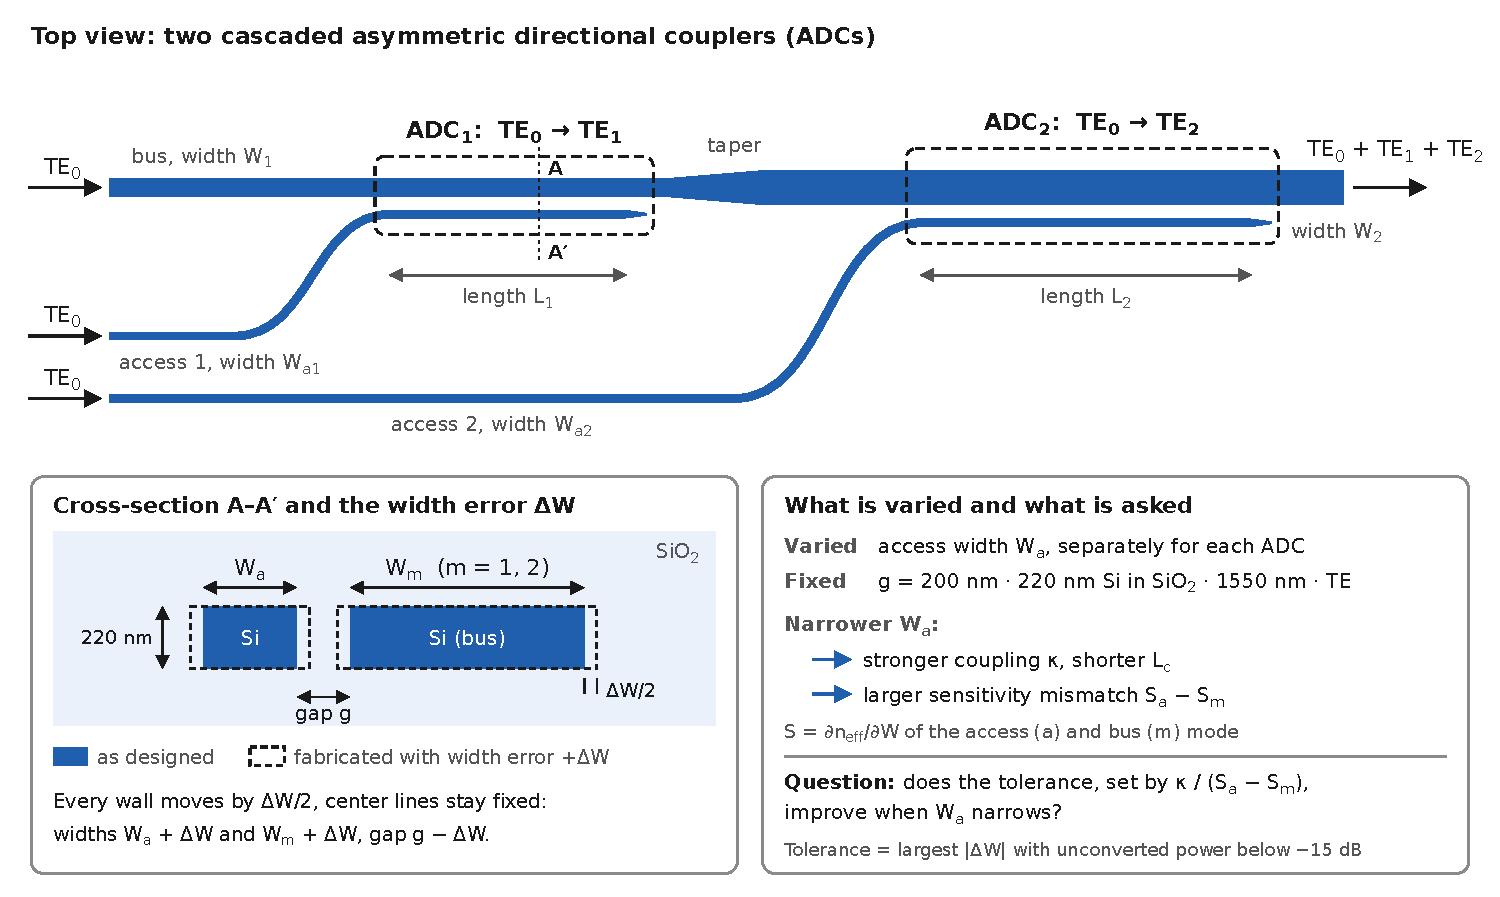
\includegraphics[width=0.74\textwidth]{figures/adc_schematic.pdf}
  \caption{The two couplers studied, in the cascaded layout of Ref.~\citep{dai2013mode}.
    Bottom left: cross-section and the uniform width error $\Delta W$ (every wall moves
    by $\Delta W/2$, centre lines fixed). Bottom right: the design variable $W_a$ and the
    question; $S = \partial n_\mathrm{eff}/\partial W$ of the access ($a$) and bus ($m$)
    mode.}
  \label{fig:schematic}
\end{figure}

% =====================================================================================
\section{Scientific background}

\paragraph{Two-mode coupled-mode theory.}
Let $n_a$ and $n_m$ be the effective indices of the access \TE{0} and bus \TE{m} modes,
each computed for its waveguide alone. In the coupled cross-section they form two
supermodes whose index difference is
\begin{equation}
  \dn_s = \sqrt{\dn_\mathrm{min}^2 + \dn_\mathrm{det}^2}, \qquad
  \dn_\mathrm{det} = n_m - n_a ,
  \label{eq:split}
\end{equation}
where $\dn_\mathrm{min} = \lambda\kappa/\pi$ expresses the coupling coefficient $\kappa$
as an index~\citep{yariv1973cmt}. Light launched into the access waveguide is converted
to the bus mode with efficiency
\begin{equation}
  \eta(L) = \left(\frac{\dn_\mathrm{min}}{\dn_s}\right)^2
            \sin^2\!\left(\frac{\pi\,\dn_s L}{\lambda}\right),
  \label{eq:eta}
\end{equation}
complete at $L_c = \lambda/(2\dn_\mathrm{min})$ when $\dn_\mathrm{det}=0$. The first
factor is the phase-matching penalty. The upper supermode carries a share
$s = \tfrac12(1-\dn_\mathrm{det}/\dn_s)$ of its power in the access mode, and at most
$4s(1-s) = (\dn_\mathrm{min}/\dn_s)^2$ can be converted: an even mixture, $s=\tfrac12$,
is the signature of phase matching.

\paragraph{Width errors and a tolerance figure of merit.}
A uniform width error detunes the coupler by $\dn_\mathrm{det} \approx (S_m - S_a)\Delta W$.
Inserted into Eq.~\eqref{eq:eta} at $L = L_c$, the unconverted power $1-\eta$ reaches
\qty{-15}{\dB} at $|\dn_\mathrm{det}| = 0.179\,\dn_\mathrm{min}$, so to first order
\begin{equation}
  \Delta W_\mathrm{tol} \approx 0.18\,\frac{\dn_\mathrm{min}}{|S_a - S_m|} .
  \label{eq:fom}
\end{equation}
Narrowing the access waveguide raises $\dn_\mathrm{min}$, but also $S_a$ and, because the
bus is then phase-matched at a lower index, $S_m$. Stronger coupling helps only if it
grows faster than the sensitivity mismatch.

\paragraph{Literature that informs the study.}
Dai et al.~\citep{dai2013mode} introduced the cascaded-ADC multiplexer, chose each bus
width so that $n_m = n_a$, and fixed the access width at \qty{0.4}{\um}, which is the
design variable here. Ding et al.~\citep{ding2013twomode} found that the coupling is most
sensitive to the narrow waveguide. Wang et al.~\citep{wang2022corrugated} shortened a
\TE{0}$\to$\TE{1} coupler on this platform from \qty{17.0}{\um} to \qty{5.6}{\um} with
sidewall corrugations and reported, without quantifying it, better robustness; their
conventional coupler is a benchmark here. García-Rodríguez et
al.~\citep{garcia2018tolerant} used a supermode analysis to find ADCs tolerant to width,
gap, height and slab-thickness variations, which supports analysing the couplers through
their supermodes.

% =====================================================================================
\section{Methodology and design}

\paragraph{Geometry and constraints.}
The platform is \qty{220}{\nm} silicon with oxide above and below, at
$\lambda = \qty{1550}{\nm}$ for TE polarization; the vertical symmetry prevents TE--TM
hybridization. The gap is fixed at $g = \qty{200}{\nm}$, as in conventional designs, so
that any gain comes from the access width alone. $W_a$ is varied from 320 to
\qty{480}{\nm}. The upper end is close to the single-mode limit: the access \TE{1} mode
appears near \qty{470}{\nm} and is only weakly guided at \qty{480}{\nm}
($n_\mathrm{eff} = 1.474$, oxide 1.444). The lower end is set by confinement and bend loss.

\paragraph{Definition of fabrication tolerance.}
A lithography or etch bias moves every sidewall, so the width error is applied to both
waveguides with fixed centre lines: $W_a\to W_a+\Delta W$, $W_m\to W_m+\Delta W$,
$g\to g-\Delta W$. The coupler keeps its nominal length $L_c$. The tolerance is the
largest $|\Delta W|$ for which $1-\eta \leq \qty{-15}{\dB}$, i.e.\ at least
\qty{97}{\percent} of the light reaches the intended mode. Errors of $\pm10$ and
$\pm\qty{20}{\nm}$ are solved, several times the wafer-scale
non-uniformity~\citep{selvaraja2010linewidth}, so that a systematic bias is also covered.

\paragraph{Numerical method.}
All modes are finite-difference solutions of 2D cross-sections in EMode2D~\citep{emode}
on a \qty{10}{\nm} grid, with \qty{1.5}{\um} of cladding beside and \qty{1}{\um} above and
below the silicon; TE fraction above 0.5 and $n_\mathrm{eff} > 1.46$ define guided TE
modes. (i) Single waveguides from 280 to \qty{1700}{\nm} give $n_a(W)$, $n_m(W)$ and $S$.
(ii) For each $W_a$, the bus width is scanned over $\pm\qty{30}{\nm}$ around isolated phase
matching and $\dn_s^2 = \dn_\mathrm{min}^2 + c^2 (W_m - W^*)^2$ is fitted, giving
$\dn_\mathrm{min}$, the bus width $W^*$ of minimum splitting, and $L_c$. (iii) For each
$\Delta W$ the scan is repeated on the perturbed geometry, and Eq.~\eqref{eq:eta} gives
$\eta(\Delta W)$, interpolated quadratically between the solved errors. (iv) The same is
done from 1500 to \qty{1600}{\nm}. (v) The access waveguide is solved in bends of 3 to
\qty{10}{\um} radius with a cylindrical bend solver and absorbing boundaries.

\paragraph{Mode-field analysis.}
Steps (ii) and (iii) use only effective indices and take $W^*$ as the phase-matched
width. To test the two-mode picture, each coupler and each of its waveguides alone are
solved on the same grid at $\Delta W = 0$ and $\pm\qty{10}{\nm}$. Each supermode is fitted
by least squares as a combination of the two single-waveguide modes at equal power. The
fit gives the access share $s$, hence $\dn_\mathrm{det} = (1-2s)\dn_s$ and $\eta$ from the
fields, and a residual: the part of the field the two modes do not explain, which would
reveal a third mode. Finally, each coupler is rebuilt with its bus at the width $W_{pm}$
where $s = \tfrac12$, and its tolerance is recomputed from the fields at $\Delta W = 0$,
$\pm5$ and $\pm\qty{10}{\nm}$.

\paragraph{Validation.}
The predictions are checked by mesh convergence (40, 20 and \qty{10}{\nm}), by an
independent open-source vector finite-difference solver
(EMpy~\citep{empy,fallahkhair2008vfd}, \qty{20}{\nm} grid, own Sellmeier models) that
reruns every step, and against the published couplers of
Refs.~\citep{wang2022corrugated,dai2013mode}.

% =====================================================================================
\section{Results and discussion}

\begin{figure}[t]
  \centering
  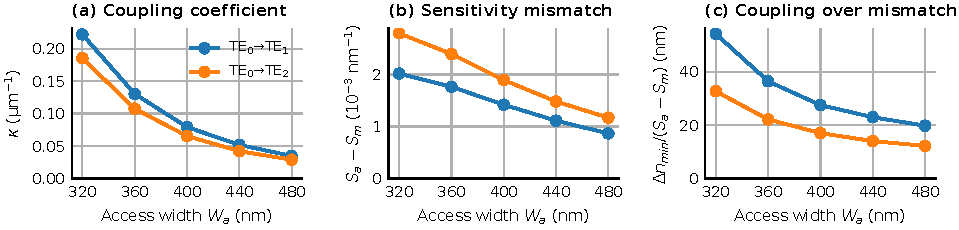
\includegraphics[width=\textwidth]{figures/report_tradeoff.pdf}
  \caption{Coupling and sensitivity against access width (EMode2D). (a) Coupling
    coefficient $\kappa = \pi\dn_\mathrm{min}/\lambda$. (b) Mismatch of the width
    sensitivities of the access and bus modes. (c) Their ratio, which sets the
    first-order tolerance, Eq.~\eqref{eq:fom}.}
  \label{fig:tradeoff}
\end{figure}

\paragraph{Coupling against sensitivity mismatch.}
From $W_a = 480$ to \qty{320}{\nm} (Fig.~\ref{fig:tradeoff}, Table~\ref{tab:designs}),
the coupling coefficient of the \TE{0}$\to$\TE{1} coupler rises from 0.035 to
\qty{0.222}{\per\um} (6.4-fold) and $L_c$ falls from 45.2 to \qty{7.1}{\um}. The
sensitivity mismatch also rises, but only from 0.87 to \qty{2.02e-3}{\per\nm}
(2.3-fold), so their ratio grows 2.7-fold. The \TE{0}$\to$\TE{2} coupler behaves the same
way (6.4-fold and 2.4-fold); its much wider bus is less sensitive to width, so its
mismatch is larger and its ratio smaller at every width. The mode fields show where the
stronger coupling comes from: at the bus wall, the intensity of the access mode alone is
\qty{-12.4}{\dB} relative to its peak for $W_a = \qty{320}{\nm}$, against
\qty{-21.0}{\dB} for \qty{480}{\nm} (Fig.~\ref{fig:fields}a).

\begin{figure}[t]
  \centering
  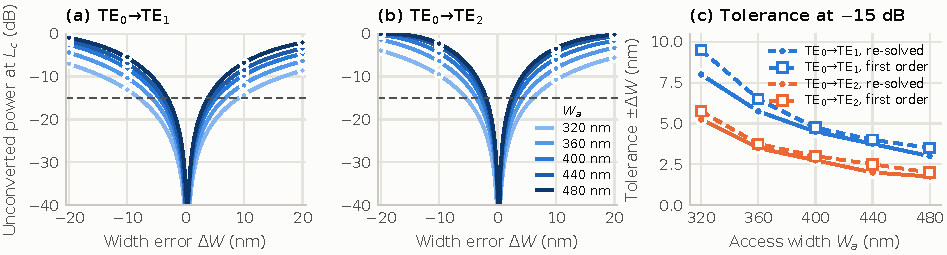
\includegraphics[width=\textwidth]{figures/report_tolerance.pdf}
  \caption{Fabrication tolerance (EMode2D and coupled-mode theory). (a, b) Unconverted
    power at the nominal length $L_c$ against the width error; dots: solved errors;
    dashed: the \qty{-15}{\dB} criterion. (c) Tolerance, re-solved and from the
    first-order estimate, Eq.~\eqref{eq:fom}.}
  \label{fig:tolerance}
\end{figure}

\paragraph{Width tolerance.}
The tolerance follows the ratio (Fig.~\ref{fig:tolerance}): it grows from
$\pm\qty{3.0}{\nm}$ at $W_a = \qty{480}{\nm}$ to $\pm\qty{8.0}{\nm}$ at \qty{320}{\nm}
for \TE{0}$\to$\TE{1}, and from $\pm1.75$ to $\pm\qty{5.25}{\nm}$ for
\TE{0}$\to$\TE{2}, which supports the hypothesis. A positive error hurts less than a
negative one, because the narrower gap strengthens the coupling and partly compensates the
detuning. Equation~\eqref{eq:fom} agrees with the re-solved values within \qty{0.5}{\nm}
except at \qty{320}{\nm} ($\pm9.5$ against $\pm\qty{8.0}{\nm}$), where the indices of the
narrow waveguides are no longer linear in width over $\pm\qty{10}{\nm}$. The
\TE{0}$\to$\TE{2} couplers with $W_a \geq \qty{400}{\nm}$ tolerate no more than about the
wafer-scale non-uniformity of \qty{2.6}{\nm}~\citep{selvaraja2010linewidth}; the
\qty{320}{\nm} couplers leave room for a systematic bias as well.

\begin{figure}[t]
  \centering
  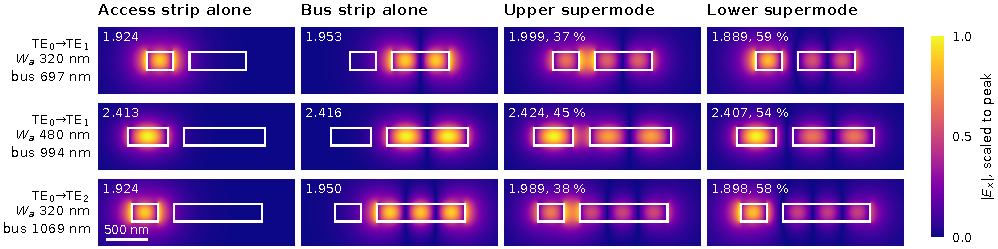
\includegraphics[width=\textwidth]{figures/report_modes.pdf}
  \caption{Mode fields (Re\,$E_x$, EMode2D) of three couplers with the bus at $W^*$: each
    waveguide alone and the two supermodes, with the silicon outlined. Numbers:
    effective index and, for the supermodes, the share of the power in the access mode.
    Upper supermodes are in phase across the gap, lower ones in anti-phase; for
    $W_a = \qty{320}{\nm}$ the mixtures are clearly uneven.}
  \label{fig:modes}
\end{figure}

\paragraph{What the mode fields add.}
The fields confirm the two-mode picture (Figs.~\ref{fig:modes} and \ref{fig:fields}).
The two single-waveguide modes explain every supermode to within \qty{2.8}{\percent} of
its field (below \qty{0.4}{\percent} at $W_a = \qty{480}{\nm}$), the upper supermode is
always in phase across the gap and the lower one in anti-phase, the TE fraction stays
above 0.93, and the splitting solved at each perturbed geometry agrees with the
index-based fits within \qty{3}{\percent}. No third mode takes part.

They also reveal what the index-based analysis missed: at $W^*$ the supermodes are not
even mixtures. The upper supermode of the \qty{320}{\nm} \TE{0}$\to$\TE{1} coupler
carries only \qty{37}{\percent} of its power in the access mode, so a coupler built at
$W^*$ converts at most $4s(1-s) = \qty{93}{\percent}$ and leaves \qty{-11.6}{\dB}
unconverted before any fabrication error (Fig.~\ref{fig:fields}c). The even-mixture width
$W_{pm}$ lies within \qty{0.5}{\nm} (\TE{0}$\to$\TE{1}) and \qty{2.5}{\nm}
(\TE{0}$\to$\TE{2}) of the width where the isolated indices are equal, the rule of
Ref.~\citep{dai2013mode}, while $W^*$ is 1.4 to \qty{12}{\nm} wider
(Fig.~\ref{fig:fields}b). The cause is that the coupling weakens as the bus widens and
confines its mode better. With $\dn_\mathrm{min}$ depending on $W_m$, Eq.~\eqref{eq:split}
has its minimum at
$W^* \approx W_{pm} - \dn_\mathrm{min}\,(\partial\dn_\mathrm{min}/\partial W_m)/S_m^2$,
an offset that grows with the coupling strength. The price of the narrow access
waveguide is thus that the phase-matching point can no longer be read off the supermode
splitting.

\begin{figure}[t]
  \centering
  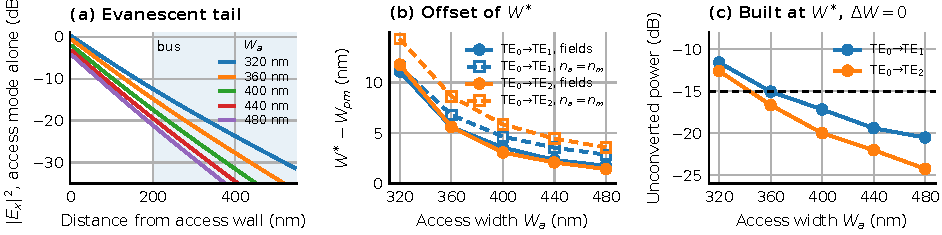
\includegraphics[width=\textwidth]{figures/report_fieldchecks.pdf}
  \caption{What the mode fields show (EMode2D). (a) Intensity of the access mode alone
    along the middle of the silicon, from its gap-side wall; the bus wall is at
    \qty{200}{\nm}. (b) Offset of $W^*$ from the phase-matched width $W_{pm}$, from the
    fields (solid) and from equal isolated indices (dashed). (c) Unconverted power of
    couplers built at $W^*$ with $\Delta W = 0$; dashed: the \qty{-15}{\dB} criterion.}
  \label{fig:fields}
\end{figure}

\paragraph{Couplers at the phase-matched width.}
Does the tolerance gain survive when each coupler is built at $W_{pm}$? This step has so
far been run only with the open-source solver. With the bus at $W_{pm}$ the supermodes are
even mixtures ($s = 0.50$--$0.51$), and the tolerance from the fields is $\pm7.5$, 6.0,
5.0, 4.0 and \qty{3.5}{\nm} for \TE{0}$\to$\TE{1} and $\pm5.0$, 3.75, 3.0, 2.5 and
\qty{2.25}{\nm} for \TE{0}$\to$\TE{2} ($W_a = 320$ to \qty{480}{\nm}), within
\qty{0.75}{\nm} of that solver's index-based values. The trend is preserved: the
tolerances of Table~\ref{tab:designs} describe phase-matched couplers, but their bus
widths should be $W_{pm}$, not $W^*$.

\begin{table}[t]
  \centering
  \caption{Couplers designed by the minimum-splitting rule (EMode2D, \qty{10}{\nm} grid).
    $W_{pm}$: phase-matched bus width from the fields. Tolerance: largest $|\Delta W|$
    with $1-\eta \leq \qty{-15}{\dB}$. $1-\eta$ at $W^*$: unconverted power of the coupler
    built at $W^*$, $\Delta W = 0$, from the fields. C-band: highest unconverted power,
    1530 to \qty{1565}{\nm}.}
  \label{tab:designs}
  \small
  \begin{tabular}{@{}rrrrrrrrrr@{}}
    \toprule
    $W_a$ & $W^*$ & $W_{pm}$ & $L_c$ & $\kappa$ & $S_a - S_m$
      & \multicolumn{2}{c}{Tolerance $\pm\Delta W$ (nm)} & $1-\eta$ at $W^*$ & C-band \\
    \cmidrule(lr){7-8}
    (nm) & (nm) & (nm) & (\unit{\um}) & (\unit{\per\um}) & (\num{e-3}/nm)
      & re-solved & first order & (dB) & (dB) \\
    \midrule
    \inputrows{generated/table_designs.tex}
    \bottomrule
  \end{tabular}
\end{table}

\paragraph{Bandwidth and bend loss.}
Over the C-band the highest unconverted power lies between \qty{-17.1}{\dB} and
\qty{-16.2}{\dB} for \TE{0}$\to$\TE{1} and between \qty{-15.8}{\dB} and \qty{-15.3}{\dB}
for \TE{0}$\to$\TE{2}, with no trend in $W_a$. A \ang{90} bend of the \qty{320}{\nm} access waveguide loses \qty{0.05}{\dB} at
\qty{3}{\um} radius and \qty{0.001}{\dB} at \qty{5}{\um}; wider waveguides lose less than
\qty{0.002}{\dB}. Contrary to the hypothesis, bend loss does not limit the access width
in the studied range for radii of \qty{5}{\um} or more.

\paragraph{Reliability.}
Refining the grid from 20 to \qty{10}{\nm} changes $L_c$ of the \qty{400}{\nm}
\TE{0}$\to$\TE{1} coupler by \qty{0.4}{\percent} (19.17, 19.74, \qty{19.82}{\um} at 40,
20, \qty{10}{\nm}) and $W^*$ by \qty{0.9}{\nm}. The independent solver reproduces every
tolerance within \qty{0.5}{\nm} (slightly higher) and the same field findings. For the
conventional \qty{400}{\nm} coupler of Ref.~\citep{wang2022corrugated}, $L_c =
\qty{19.8}{\um}$ against their \qty{17.0}{\um}, which refers to the straight section only;
the S-bends, not modelled here, add coupling. For the \TM{0}$\to$\TM{1} coupler of
Ref.~\citep{dai2013mode} the isolated phase-matching bus width is \qty{1035}{\nm} against
their \qty{1020}{\nm}.

\paragraph{Limitations.}
Only 2D cross-sections are solved: coupling in the S-bends, the bus tapers and
reflections are not modelled, so a real coupler needs a shorter straight section than
$L_c$. Only uniform width errors are studied; thickness, sidewall angle and gap-only
errors also vary. Scattering loss, which grows as the access waveguide narrows, is not
included. The unconverted power is a coupler-level figure: the crosstalk of a complete
multiplexer needs a propagation simulation (EME or FDTD) and remains to be tested.

% =====================================================================================
\section{Conclusion}

A narrower access waveguide makes a silicon ADC more tolerant to width errors: from
$W_a = 480$ to \qty{320}{\nm} the tolerance grows 2.7-fold for \TE{0}$\to$\TE{1}
($\pm3.0$ to $\pm\qty{8.0}{\nm}$) and 3-fold for \TE{0}$\to$\TE{2} ($\pm1.75$ to
$\pm\qty{5.25}{\nm}$). Stronger coupling alone does not guarantee this: the coupling grows
6.4-fold, the sensitivity mismatch 2.3-fold, and the tolerance follows their ratio. The
mode fields confirm the two-mode mechanism and trace the gain to the stronger evanescent
field of the narrow access mode at the bus. They also show that strong coupling moves the
minimum of the supermode splitting up to \qty{12}{\nm} away from phase matching, enough to
leave about \qty{-12}{\dB} unconverted before any fabrication error. The bus width must
therefore come from equal isolated indices or the field-based even mixture; with that
rule, the tolerance gain is preserved in the cross-check. Open questions are the
EMode2D run at the phase-matched width, full 3D simulations including the S-bends,
thickness and sidewall-angle variations, scattering loss, and the crosstalk of a complete
multiplexer.

{\small
\bibliographystyle{unsrtnat}
\bibliography{references}
}

\end{document}
